\chapter{Enunciado do problema}\label{chp:introducao} 
Qual será o problema tratado pelo projeto e qual sua importância? Qual será a contribuição para a área se bem sucedido? Cite trabalhos relevantes na área, conforme necessário.

Eis um exemplo de citação \cite{Gradvohl2014}. Ou, conforme \textcite{Gradvohl2014}, um exemplo de citação em linha.

Veja, na Figura~\ref{fig:supercomputador} a seguir, um exemplo de adição de figura no texto. Note que é preciso definir um rótulo (\textit{label}) dentro do comando de definição da figura.

\begin{figure}[!htb]
    \centering
    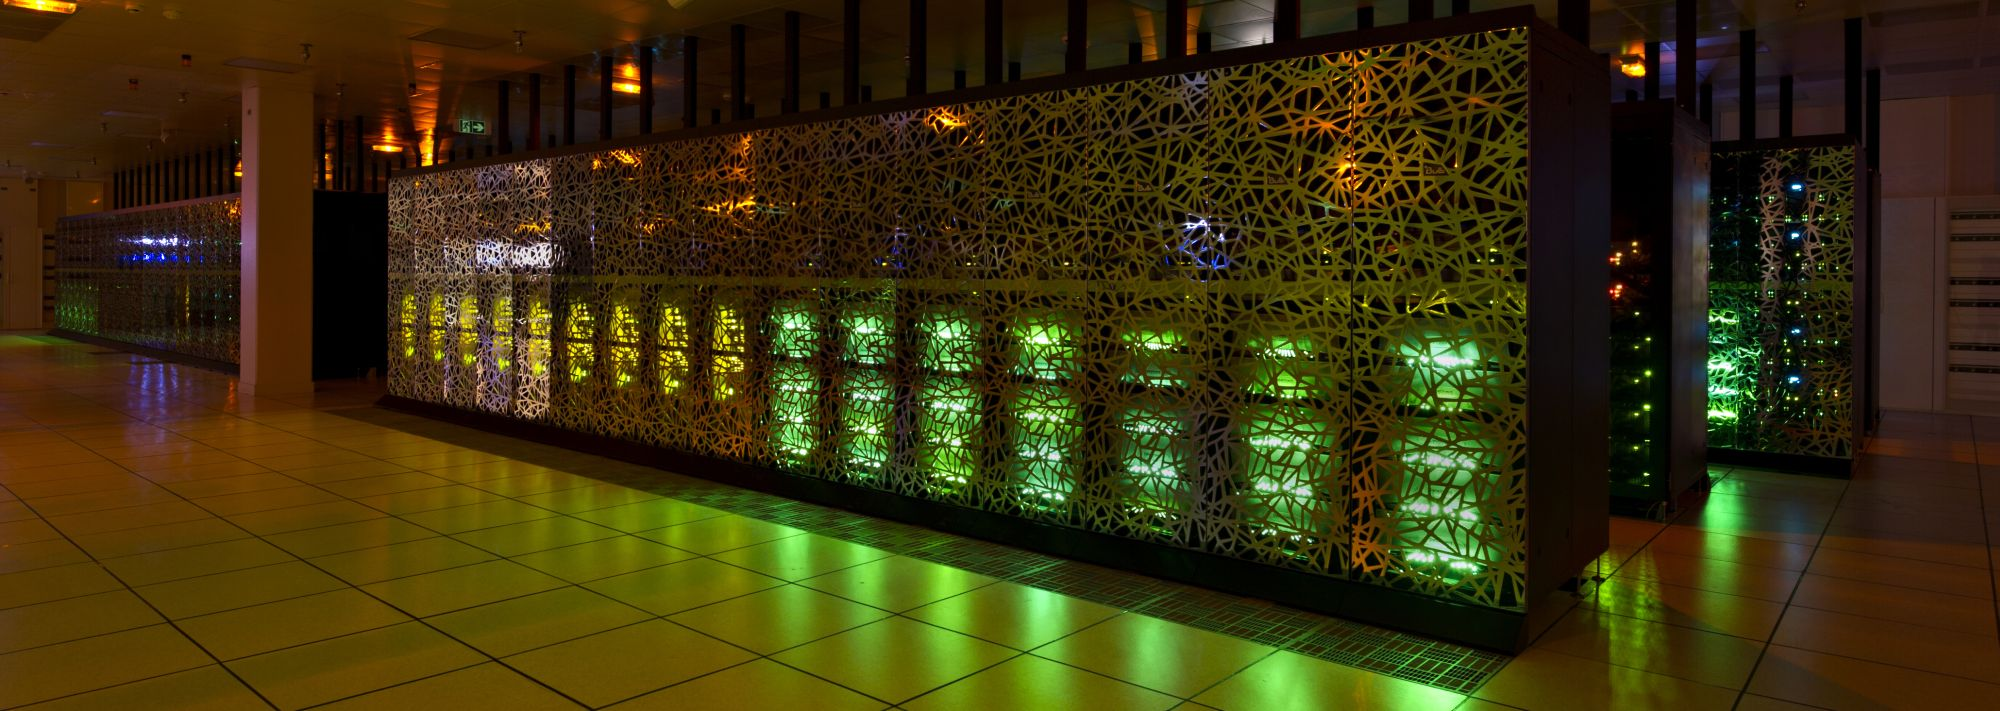
\includegraphics[width=.9\textwidth]{figuras/Supercomputer.jpg}
    \caption{Exemplo de figura embutida no texto}
    \label{fig:supercomputador}
\end{figure}

Aqui um exemplo de como referenciar a Tabela~\ref{tab:tabela_1}. Note que é preciso definir um rótulo (\textit{label}) dentro do comando de definição da tabela.

% Veja a seguir um exemplo de Tabela.
% Você pode usar o site http://www.tablesgenerator.com
% para gerar as tabelas em LaTeX.
\begin{table}[!htp]
\caption[Legenda curta da tabela]{Legenda longa e mais detalhada da tabela.}
\label{tab:tabela_1}
\begin{center}
\begin{tabular}{cc}
\toprule % Linha superior
Coluna 1 & Coluna2 \\ \midrule % Linha do meio 
a & b \\
c & d \\
e & f \\\bottomrule % Linha inferior
\end{tabular}
\end{center}
\end{table}